
%% bare_conf.tex
%% V1.4b
%% 2015/08/26
%% by Michael Shell
%% See:
%% http://www.michaelshell.org/
%% for current contact information.
%%
%% This is a skeleton file demonstrating the use of IEEEtran.cls
%% (requires IEEEtran.cls version 1.8b or later) with an IEEE
%% conference paper.
%%
%% Support sites:
%% http://www.michaelshell.org/tex/ieeetran/
%% http://www.ctan.org/pkg/ieeetran
%% and
%% http://www.ieee.org/

%%*************************************************************************
%% Legal Notice:
%% This code is offered as-is without any warranty either expressed or
%% implied; without even the implied warranty of MERCHANTABILITY or
%% FITNESS FOR A PARTICULAR PURPOSE! 
%% User assumes all risk.
%% In no event shall the IEEE or any contributor to this code be liable for
%% any damages or losses, including, but not limited to, incidental,
%% consequential, or any other damages, resulting from the use or misuse
%% of any information contained here.
%%
%% All comments are the opinions of their respective authors and are not
%% necessarily endorsed by the IEEE.
%%
%% This work is distributed under the LaTeX Project Public License (LPPL)
%% ( http://www.latex-project.org/ ) version 1.3, and may be freely used,
%% distributed and modified. A copy of the LPPL, version 1.3, is included
%% in the base LaTeX documentation of all distributions of LaTeX released
%% 2003/12/01 or later.
%% Retain all contribution notices and credits.
%% ** Modified files should be clearly indicated as such, including  **
%% ** renaming them and changing author support contact information. **
%%*************************************************************************


% *** Authors should verify (and, if needed, correct) their LaTeX system  ***
% *** with the testflow diagnostic prior to trusting their LaTeX platform ***
% *** with production work. The IEEE's font choices and paper sizes can   ***
% *** trigger bugs that do not appear when using other class files.       ***                          ***
% The testflow support page is at:
% http://www.michaelshell.org/tex/testflow/



\documentclass[conference]{IEEEtran}

\usepackage[utf8]{inputenc}
\usepackage{graphicx}
\graphicspath{ {images/} }

% Some Computer Society conferences also require the compsoc mode option,
% but others use the standard conference format.
%
% If IEEEtran.cls has not been installed into the LaTeX system files,
% manually specify the path to it like:
% \documentclass[conference]{../sty/IEEEtran}





% Some very useful LaTeX packages include:
% (uncomment the ones you want to load)


% *** MISC UTILITY PACKAGES ***
%
%\usepackage{ifpdf}
% Heiko Oberdiek's ifpdf.sty is very useful if you need conditional
% compilation based on whether the output is pdf or dvi.
% usage:
% \ifpdf
%   % pdf code
% \else
%   % dvi code
% \fi
% The latest version of ifpdf.sty can be obtained from:
% http://www.ctan.org/pkg/ifpdf
% Also, note that IEEEtran.cls V1.7 and later provides a builtin
% \ifCLASSINFOpdf conditional that works the same way.
% When switching from latex to pdflatex and vice-versa, the compiler may
% have to be run twice to clear warning/error messages.



\usepackage[tableposition=top]{caption}
\usepackage[hidelinks]{hyperref}
\usepackage{lineno,amsmath,algorithm,algpseudocode}
\modulolinenumbers[1]
\usepackage{graphicx}
\usepackage{caption}
\usepackage{subcaption}
\usepackage{booktabs}
\newcommand{\head}[1]{\textnormal{\textbf{#1}}}


% *** CITATION PACKAGES ***
%
%\usepackage{cite}
% cite.sty was written by Donald Arseneau
% V1.6 and later of IEEEtran pre-defines the format of the cite.sty package
% \cite{} output to follow that of the IEEE. Loading the cite package will
% result in citation numbers being automatically sorted and properly
% "compressed/ranged". e.g., [1], [9], [2], [7], [5], [6] without using
% cite.sty will become [1], [2], [5]--[7], [9] using cite.sty. cite.sty's
% \cite will automatically add leading space, if needed. Use cite.sty's
% noadjust option (cite.sty V3.8 and later) if you want to turn this off
% such as if a citation ever needs to be enclosed in parenthesis.
% cite.sty is already installed on most LaTeX systems. Be sure and use
% version 5.0 (2009-03-20) and later if using hyperref.sty.
% The latest version can be obtained at:
% http://www.ctan.org/pkg/cite
% The documentation is contained in the cite.sty file itself.






% *** GRAPHICS RELATED PACKAGES ***
%
\ifCLASSINFOpdf
  % \usepackage[pdftex]{graphicx}
  % declare the path(s) where your graphic files are
  % \graphicspath{{../pdf/}{../jpeg/}}
  % and their extensions so you won't have to specify these with
  % every instance of \includegraphics
  % \DeclareGraphicsExtensions{.pdf,.jpeg,.png}
\else
  % or other class option (dvipsone, dvipdf, if not using dvips). graphicx
  % will default to the driver specified in the system graphics.cfg if no
  % driver is specified.
  % \usepackage[dvips]{graphicx}
  % declare the path(s) where your graphic files are
  % \graphicspath{{../eps/}}
  % and their extensions so you won't have to specify these with
  % every instance of \includegraphics
  % \DeclareGraphicsExtensions{.eps}
\fi
% graphicx was written by David Carlisle and Sebastian Rahtz. It is
% required if you want graphics, photos, etc. graphicx.sty is already
% installed on most LaTeX systems. The latest version and documentation
% can be obtained at: 
% http://www.ctan.org/pkg/graphicx
% Another good source of documentation is "Using Imported Graphics in
% LaTeX2e" by Keith Reckdahl which can be found at:
% http://www.ctan.org/pkg/epslatex
%
% latex, and pdflatex in dvi mode, support graphics in encapsulated
% postscript (.eps) format. pdflatex in pdf mode supports graphics
% in .pdf, .jpeg, .png and .mps (metapost) formats. Users should ensure
% that all non-photo figures use a vector format (.eps, .pdf, .mps) and
% not a bitmapped formats (.jpeg, .png). The IEEE frowns on bitmapped formats
% which can result in "jaggedy"/blurry rendering of lines and letters as
% well as large increases in file sizes.
%
% You can find documentation about the pdfTeX application at:
% http://www.tug.org/applications/pdftex





% *** MATH PACKAGES ***
%
%\usepackage{amsmath}
% A popular package from the American Mathematical Society that provides
% many useful and powerful commands for dealing with mathematics.
%
% Note that the amsmath package sets \interdisplaylinepenalty to 10000
% thus preventing page breaks from occurring within multiline equations. Use:
%\interdisplaylinepenalty=2500
% after loading amsmath to restore such page breaks as IEEEtran.cls normally
% does. amsmath.sty is already installed on most LaTeX systems. The latest
% version and documentation can be obtained at:
% http://www.ctan.org/pkg/amsmath





% *** SPECIALIZED LIST PACKAGES ***
%
%\usepackage{algorithmic}
% algorithmic.sty was written by Peter Williams and Rogerio Brito.
% This package provides an algorithmic environment fo describing algorithms.
% You can use the algorithmic environment in-text or within a figure
% environment to provide for a floating algorithm. Do NOT use the algorithm
% floating environment provided by algorithm.sty (by the same authors) or
% algorithm2e.sty (by Christophe Fiorio) as the IEEE does not use dedicated
% algorithm float types and packages that provide these will not provide
% correct IEEE style captions. The latest version and documentation of
% algorithmic.sty can be obtained at:
% http://www.ctan.org/pkg/algorithms
% Also of interest may be the (relatively newer and more customizable)
% algorithmicx.sty package by Szasz Janos:
% http://www.ctan.org/pkg/algorithmicx




% *** ALIGNMENT PACKAGES ***
%
%\usepackage{array}
% Frank Mittelbach's and David Carlisle's array.sty patches and improves
% the standard LaTeX2e array and tabular environments to provide better
% appearance and additional user controls. As the default LaTeX2e table
% generation code is lacking to the point of almost being broken with
% respect to the quality of the end results, all users are strongly
% advised to use an enhanced (at the very least that provided by array.sty)
% set of table tools. array.sty is already installed on most systems. The
% latest version and documentation can be obtained at:
% http://www.ctan.org/pkg/array


% IEEEtran contains the IEEEeqnarray family of commands that can be used to
% generate multiline equations as well as matrices, tables, etc., of high
% quality.




% *** SUBFIGURE PACKAGES ***
%\ifCLASSOPTIONcompsoc
%  \usepackage[caption=false,font=normalsize,labelfont=sf,textfont=sf]{subfig}
%\else
%  \usepackage[caption=false,font=footnotesize]{subfig}
%\fi
% subfig.sty, written by Steven Douglas Cochran, is the modern replacement
% for subfigure.sty, the latter of which is no longer maintained and is
% incompatible with some LaTeX packages including fixltx2e. However,
% subfig.sty requires and automatically loads Axel Sommerfeldt's caption.sty
% which will override IEEEtran.cls' handling of captions and this will result
% in non-IEEE style figure/table captions. To prevent this problem, be sure
% and invoke subfig.sty's "caption=false" package option (available since
% subfig.sty version 1.3, 2005/06/28) as this is will preserve IEEEtran.cls
% handling of captions.
% Note that the Computer Society format requires a larger sans serif font
% than the serif footnote size font used in traditional IEEE formatting
% and thus the need to invoke different subfig.sty package options depending
% on whether compsoc mode has been enabled.
%
% The latest version and documentation of subfig.sty can be obtained at:
% http://www.ctan.org/pkg/subfig




% *** FLOAT PACKAGES ***
%
%\usepackage{fixltx2e}
% fixltx2e, the successor to the earlier fix2col.sty, was written by
% Frank Mittelbach and David Carlisle. This package corrects a few problems
% in the LaTeX2e kernel, the most notable of which is that in current
% LaTeX2e releases, the ordering of single and double column floats is not
% guaranteed to be preserved. Thus, an unpatched LaTeX2e can allow a
% single column figure to be placed prior to an earlier double column
% figure.
% Be aware that LaTeX2e kernels dated 2015 and later have fixltx2e.sty's
% corrections already built into the system in which case a warning will
% be issued if an attempt is made to load fixltx2e.sty as it is no longer
% needed.
% The latest version and documentation can be found at:
% http://www.ctan.org/pkg/fixltx2e


%\usepackage{stfloats}
% stfloats.sty was written by Sigitas Tolusis. This package gives LaTeX2e
% the ability to do double column floats at the bottom of the page as well
% as the top. (e.g., "\begin{figure*}[!b]" is not normally possible in
% LaTeX2e). It also provides a command:
%\fnbelowfloat
% to enable the placement of footnotes below bottom floats (the standard
% LaTeX2e kernel puts them above bottom floats). This is an invasive package
% which rewrites many portions of the LaTeX2e float routines. It may not work
% with other packages that modify the LaTeX2e float routines. The latest
% version and documentation can be obtained at:
% http://www.ctan.org/pkg/stfloats
% Do not use the stfloats baselinefloat ability as the IEEE does not allow
% \baselineskip to stretch. Authors submitting work to the IEEE should note
% that the IEEE rarely uses double column equations and that authors should try
% to avoid such use. Do not be tempted to use the cuted.sty or midfloat.sty
% packages (also by Sigitas Tolusis) as the IEEE does not format its papers in
% such ways.
% Do not attempt to use stfloats with fixltx2e as they are incompatible.
% Instead, use Morten Hogholm'a dblfloatfix which combines the features
% of both fixltx2e and stfloats:
%
% \usepackage{dblfloatfix}
% The latest version can be found at:
% http://www.ctan.org/pkg/dblfloatfix




% *** PDF, URL AND HYPERLINK PACKAGES ***
%
%\usepackage{url}
% url.sty was written by Donald Arseneau. It provides better support for
% handling and breaking URLs. url.sty is already installed on most LaTeX
% systems. The latest version and documentation can be obtained at:
% http://www.ctan.org/pkg/url
% Basically, \url{my_url_here}.




% *** Do not adjust lengths that control margins, column widths, etc. ***
% *** Do not use packages that alter fonts (such as pslatex).         ***
% There should be no need to do such things with IEEEtran.cls V1.6 and later.
% (Unless specifically asked to do so by the journal or conference you plan
% to submit to, of course. )


% correct bad hyphenation here
\hyphenation{op-tical net-works semi-conduc-tor}


\begin{document}
%
% paper title
% Titles are generally capitalized except for words such as a, an, and, as,
% at, but, by, for, in, nor, of, on, or, the, to and up, which are usually
% not capitalized unless they are the first or last word of the title.
% Linebreaks \\ can be used within to get better formatting as desired.
% Do not put math or special symbols in the title.
\title{Distributed Leader Optimization}


% author names and affiliations
% use a multiple column layout for up to three different
% affiliations
\author{\IEEEauthorblockN{Author 01}
\IEEEauthorblockA{School of Electrical and\\Computer Engineering\\
Georgia Institute of Technology\\
Atlanta, Georgia 30332--0250\\
Email: http://www.michaelshell.org/contact.html}
\and
\IEEEauthorblockN{Author 02}
\IEEEauthorblockA{Twentieth Century Fox\\
Springfield, USA\\
Email: homer@thesimpsons.com}
\and
\IEEEauthorblockN{Author 03}
\IEEEauthorblockA{Starfleet Academy\\
San Francisco, California 96678--2391\\
Telephone: (800) 555--1212\\
Fax: (888) 555--1212}}

% conference papers do not typically use \thanks and this command
% is locked out in conference mode. If really needed, such as for
% the acknowledgment of grants, issue a \IEEEoverridecommandlockouts
% after \documentclass

% for over three affiliations, or if they all won't fit within the width
% of the page, use this alternative format:
% 
%\author{\IEEEauthorblockN{Michael Shell\IEEEauthorrefmark{1},
%Homer Simpson\IEEEauthorrefmark{2},
%James Kirk\IEEEauthorrefmark{3}, 
%Montgomery Scott\IEEEauthorrefmark{3} and
%Eldon Tyrell\IEEEauthorrefmark{4}}
%\IEEEauthorblockA{\IEEEauthorrefmark{1}School of Electrical and Computer Engineering\\
%Georgia Institute of Technology,
%Atlanta, Georgia 30332--0250\\ Email: see http://www.michaelshell.org/contact.html}
%\IEEEauthorblockA{\IEEEauthorrefmark{2}Twentieth Century Fox, Springfield, USA\\
%Email: homer@thesimpsons.com}
%\IEEEauthorblockA{\IEEEauthorrefmark{3}Starfleet Academy, San Francisco, California 96678-2391\\
%Telephone: (800) 555--1212, Fax: (888) 555--1212}
%\IEEEauthorblockA{\IEEEauthorrefmark{4}Tyrell Inc., 123 Replicant Street, Los Angeles, California 90210--4321}}




% use for special paper notices
%\IEEEspecialpapernotice{(Invited Paper)}




% make the title area
\maketitle

% As a general rule, do not put math, special symbols or citations
% in the abstract
\begin{abstract}
Operational maturity of biological control systems have fuelled the inspiration for a large number of mathematical and logical models for control, automation and optimisation. The human brain represents the most sophisticated control architecture known to us and is a central motivation for several research attempts across various domains. In the present work, we introduce an algorithm for mathematical optimisation that derives its intuition from the hierarchical and distributed operations of the human motor system. The system comprises global leaders, local leaders and an effector population that adapt dynamically to attain global optimisation via a feedback mechanism coupled with the structural hierarchy. The hierarchical system operation is distributed into local control for movement and global controllers that facilitate gross motion and decision making. We present our algorithm as a variant of the classical Differential Evolution algorithm, introducing a hierarchical crossover operation. The discussed approach is tested exhaustively on standard test functions as well as the CEC 2017 benchmark. Our algorithm significantly outperforms various standard algorithms as well as their popular variants as discussed in the results.
\end{abstract}

% no keywords




% For peer review papers, you can put extra information on the cover
% page as needed:
% \ifCLASSOPTIONpeerreview
% \begin{center} \bfseries EDICS Category: 3-BBND \end{center}
% \fi
%
% For peerreview papers, this IEEEtran command inserts a page break and
% creates the second title. It will be ignored for other modes.
\IEEEpeerreviewmaketitle



\section{Introduction}
% no \IEEEPARstart
Operational maturity of biological control systems have enamored researchers across various domains. Consequently, they have been the source of inspiration of mathematical and logical models for control, automation and optimization. At the cellular and organ levels, In the E.Coli bacterium, there is sensing and locomotion involved in seeking nourishment and avoiding harmful chemicals. There is sensing via the recognition of chemicals, internal decision making and actuation via locomotion. These behavioural characteristics have fueled the inspiration for the Bacterial Foraging Optimization Algorithm.\\

The function of human brain is at the pinnacle of relevance at the current social and technological standing, and several research initiatives have been attempting to mimic human-like precision, accuracy and efficiency. The brain has developed amazing performance in several day-to-day tasks such as grasping, walking etc. which happens due to the parallel work and management of brain sections governing various steps involved in completion of a task. The brain function activities can be categorised in 2 broad categories: sensory and motor operations. Sensory cortical functions have inspired the concepts of neural networks and deep learning which have already been successfully scaled to solve a vast amount of problems.

While not always the case, it is at times useful and accurate to view a biological neural system to be arranged in a hierarchical fashion. One part of the brin that is clearly hierarchical is the human motor system. It is a hierarchical and distributed control system. It can be classified as having local control functions for movement and higher level controllers that control gross motion and decision making involved in planning actions. It is connected to many parts of the brain, so that we can plan, learn and execute motions or actions. The motor learning sequence of operations involves an adaptive model building in attaining optimal co-ordination of motion. The hierarchy of motor operations can be represented as the following steps:
\begin{itemize}
	\item[1.] Motivation and planning of the action.
	\item[2.] Generation of instructions for movement.
	\item[3.] Refinement of instructions based on feedback.
	\item[4.] Maintenance of posture and smooth execution of actions.
\end{itemize}
Signal detection in the somatosensory cortex area, that pertains to touch sense, can participate as a possible motivator for the initiation of motor actions. Motor control is a type of neural hierarchical distributed learning control system. The neurons interface via special cells to the sensory inputs and are also control systems so that we can move our arms and legs via the neuronal control of muscle contraction and expansioin.

The human motor function represents a distributed and hierarchical system. The optimal execution involves distributed brain structures at different levels of hierarchy. These include the pre-frontal cortex, motor cortex, spinal cord, the anterior horn cells etc. in generating action sequences, a sequence of actions is implemented by a string of subsequences of actions, each possibly implemented in a different part of the body. The optimization of the motor learning procedure takes place at multiple levels of hierarchy:

\includegraphics[scale=0.6]{motorControl}

\begin{itemize}
\item[1.] Stage 1 involves motivation and planning for the action to be performed. This may be categorised as involving collaboration of the sensory and the pre-motor components. For instance, signals in the somatosensory cortex area, pertaining to the sense of touch may trigger a chain of motor actions. For voluntary motor actions, decision making and planning occurs in the pre-frontal cortex and the  pyramidal cells of the motor cortex.

\item[2.] These global leaders then pass the information to the anterior horn cells in the spinal cord. These cells represent the local leaders and govern the operations of a set of effectors.

\item[3.] For optimality of all actions, neurons act in unison. The neurons in the motor cortex act like global leaders and send inhibitory influence over the anterior horn cells (local leaders) located in the spinal cord. These local leaders are connected to the muscle fibre (effectors) through a peripheral nerve and neuromuscular junction.

\item[4.] Whenever, a person plans to perform an action, the electrical signals generated from the pyramidal neurons in the motor cortex (representing the decision making process) are transmitted via a supraspinal tract on the anterior horn cells (communicating to the local leaders). Initially, send inhibitory influence to the population over the local leaders. Efficient execution of task requires feedback based faciliation and inhibition of the effectors. These result in contraction of the antagonist and relaxation of the agonist muscle fibres through the local leaders.

\item[5.] This sequence of updation of the constituent particles characteristics, categories Stage 4, representing the optimaal convergence of the system leading to smooth motor execution (enjoy the coffee!).
\end{itemize}

The prefrontal cortex and motor cortex combined, represent the frontal cortex and constitute the action based decision making process, or in conjunction, what we call the global leader.


\section{Classical Differential Evolution}

The classical Differential Evolution (DE) algorithm is a population-based global optimization algorithm, utilizing a crossover and mmutation approach to generate new individuals in the population for achieving optimum solutions. For each individual $x_i$ that belongs to the population, DE randomly samples three other individuals from the population $a_i$, $b_i$ and $c_i$. Then using the randomly chosen points, a new individual vector is generated using equation \eqref{de}:

\begin{equation}
\label{de}
u_i = a_i + F (b_i - c_i)
\end{equation}

Where, $F$ is called the differential weight (Usually lies between $[0, 1]$).\\
And to obtain the new position of the individual, a crossover operation is implemented between $x_i$ and $u_i$, controlled by the parameter $CR$ called the crossover probability. The value for $CR$ always lies between $[0, 1]$.

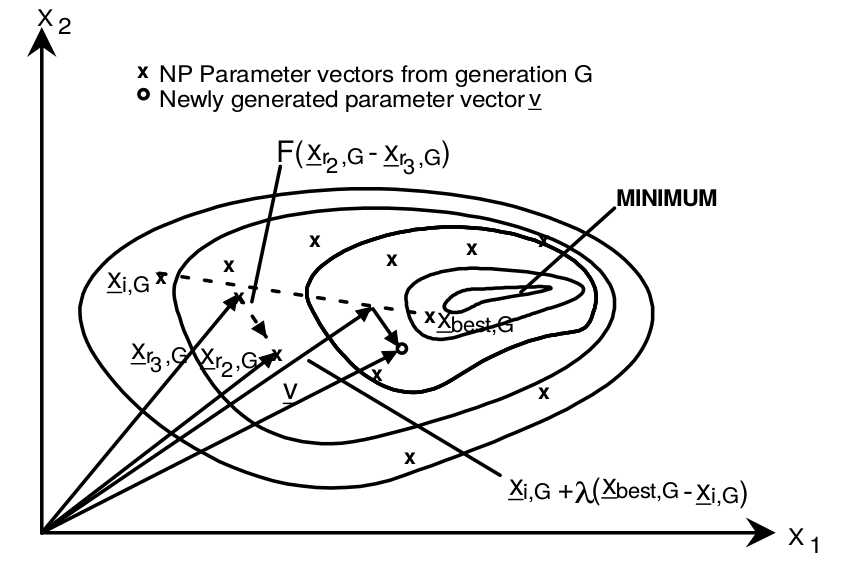
\includegraphics[scale=0.3]{contourDE}

%\begin{algorithm}
%\caption{Classical Differential Evolution}
%\label{algo}
%\begin{algorithmic}[1]
%	\Procedure{Start}{}
%		\State Initialize parameters ($HC$, $P$, $N_l$, $N$).
%		\State Generate initial global leader $g_L$ as a random point.
%		\State Generate $N_l$ local leader points around $g_L$.
%		\State Using a Normal distribution, generate $N$ points for population $P$ around the local leaders.
%		\While{termination criteria is not met}
%		%%%%%%%%%%%%%%%%%%%%%%%%%%%%%%%%%%%%%%%%%%%%%%%%%%%%%%%%%%%%%%%%%%%%%%%%%%%%%%%%%%%%%%
%			\For{each individual $x_i$ in $P$}
%				\State compute the corresponding local leader $l$ based on nearest position.
%				\State Let $u = 0$ be an empty vector.
%				\State Let $i_c$ and $i_N$ be the current generation and total generations of the procedure.
%				\If {$i_c \textless (HC*i_N)$}
%					\State $u = E_g$ from \eqref{one}.
%				\Else
%					\State $u = E_l$ from \eqref{two} 
%				\EndIf
%				
%				\For{each dimension $i$}
%					\State Generate $r_i = U(0, 1)$, a random number between 0 and 1.
%					\If {$r_i \textless HC$}
%						\State Set $x_i^{'} = x_i$.
%					\Else
%						\State Set $x_i^{'} = u_i$
%					\EndIf
%				\EndFor
%				\If {$f(x^{'}) \textless f(x)$}
%					\State Replace $x$ with $x^{'}$ in the population.
%				\EndIf
%			\EndFor
%			\State Alter local leaders in each population cluster based on objective function value.
%			\State Compute updated global leader $g_L$.
%		\EndWhile
%	\EndProcedure
%\end{algorithmic}
%\end{algorithm}

\section{Distributed Leader Optimization}
Taking inspiration from the human motor system, we model the hierarchical motor operations in our optimization agents, where we define a global leader which influences the action of several distributed local leaders and the particle agents which act as the effectors. The global leader is analogous to the decision making and planning section in the motor system hierarchy whilst, the local leaders correspond to motion generators acting under the influence of the  global leader.

The position of each particle in the population is affected by the influence of global leaders and local leaders, while also being affected by a randomly chosen particle from the population to induce some stochasticity in the optimization pipeline. We first model the influence of the global leader on the local leaders and the influences of the local leaders  on each population element using equation \eqref{one} and \eqref{two}. We introduce a hierarchical crossover between the two influencing equations governed by a hierarchical crossover parameter $HC$.

Analogously to [step 3] in the brain motor operation, the updation of particle positions requires generating feedback for the leaders as a part of the optimization procedure, and hence the local leaders and the global leader are updated based onn their objective function value generated from the perturbations in population particles. This series of events comprise of one optimization pass (one loop step). On execution of several optimization passes as described, the system is able to converge to an optimal configuration, analogous to the successful execution of the required task as shown in [step 4].

The updated position of the particle $x$ is governed by the hierarchical crossover operation and a mutation operation. The hierarchical operation is affected by the global leader $g_L$ and the local leader $l$ through the parametric equations \eqref{one} and \eqref{two}. Switching between the two is governed by the hierarchical crossover parameter $HC$. The given equations are discussed as follows:

\begin{equation}
\label{one}
E_g = g_L + F (l - c)
\end{equation}

\begin{equation}
\label{two}
E_l = l + F (x - c)
\end{equation}

\begin{algorithm}
\caption{Distributed Leader Optimization}
\label{algo}
\begin{algorithmic}[1]
	\Procedure{Start}{}
		\State Initialize parameters ($HC$, $P$, $N_l$, $N$).
		\State Generate initial global leader $g_L$ as a random point.
		\State Generate $N_l$ local leader points around $g_L$.
		\State Using a Normal distribution, generate $N$ points for population $P$ around the local leaders.
		\While{termination criteria is not met}
		%%%%%%%%%%%%%%%%%%%%%%%%%%%%%%%%%%%%%%%%%%%%%%%%%%%%%%%%%%%%%%%%%%%%%%%%%%%%%%%%%%%%%%
			\For{each individual $x_i$ in $P$}
				\State compute the corresponding local leader $l$ based on nearest position.
				\State Let $u = 0$ be an empty vector.
				\State Let $i_c$ and $i_N$ be the current generation and total generations of the procedure.
				\If {$i_c \textless (HC*i_N)$}
					\State $u = E_g$ from \eqref{one}.
				\Else
					\State $u = E_l$ from \eqref{two}.
				\EndIf
				
				\For{each dimension $i$}
					\State Generate $r_i = U(0, 1)$, a random number between 0 and 1.
					\If {$r_i \textless HC$}
						\State Set $x_i^{'} = x_i$.
					\Else
						\State Set $x_i^{'} = u_i$
					\EndIf
				\EndFor
				\If {$f(x^{'}) \textless f(x)$}
					\State Replace $x$ with $x^{'}$ in the population.
				\EndIf
			\EndFor
			\State Alter local leaders in each population cluster based on objective function value.
			\State Compute updated global leader $g_L$.
		\EndWhile
	\EndProcedure
\end{algorithmic}
\end{algorithm}

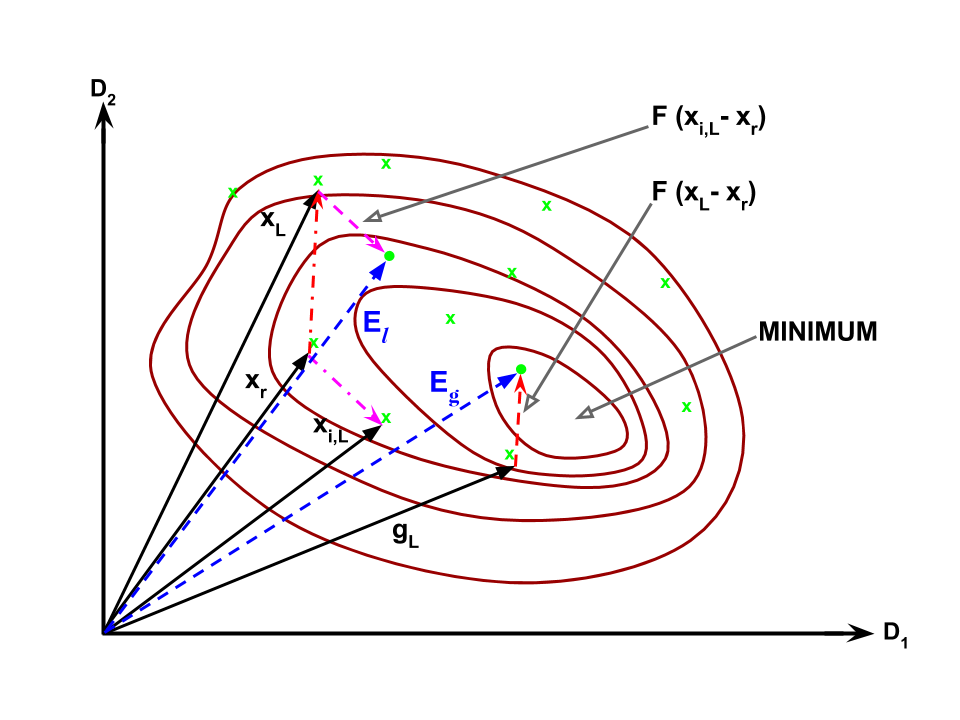
\includegraphics[scale=0.25]{contourDL}

In the algorithm \ref{algo}, The Hierarchical crossover is controlled by the conditional equation $i_c \textless (HC*i_N)$. According to this equation, during the initial phases ($HC$ fraction of total generations) of the optimization procedure, only the local leader is responsible for the motion of the agents, and after a certain amount of time has passed, the global leader also takes part in the motion generation process, signifying the motor control operation.
Additionaly, The hierarchical crossover parameter $HC$ also influences the mutation process wherein the degree of final mutation is decided based on the probability $HC$.


% An example of a floating figure using the graphicx package.
% Note that \label must occur AFTER (or within) \caption.
% For figures, \caption should occur after the \includegraphics.
% Note that IEEEtran v1.7 and later has special internal code that
% is designed to preserve the operation of \label within \caption
% even when the captionsoff option is in effect. However, because
% of issues like this, it may be the safest practice to put all your
% \label just after \caption rather than within \caption{}.
%
% Reminder: the "draftcls" or "draftclsnofoot", not "draft", class
% option should be used if it is desired that the figures are to be
% displayed while in draft mode.
%
%\begin{figure}[!t]
%\centering
%\includegraphics[width=2.5in]{myfigure}
% where an .eps filename suffix will be assumed under latex, 
% and a .pdf suffix will be assumed for pdflatex; or what has been declared
% via \DeclareGraphicsExtensions.
%\caption{Simulation results for the network.}
%\label{fig_sim}
%\end{figure}

% Note that the IEEE typically puts floats only at the top, even when this
% results in a large percentage of a column being occupied by floats.


% An example of a double column floating figure using two subfigures.
% (The subfig.sty package must be loaded for this to work.)
% The subfigure \label commands are set within each subfloat command,
% and the \label for the overall figure must come after \caption.
% \hfil is used as a separator to get equal spacing.
% Watch out that the combined width of all the subfigures on a 
% line do not exceed the text width or a line break will occur.
%
%\begin{figure*}[!t]
%\centering
%\subfloat[Case I]{\includegraphics[width=2.5in]{box}%
%\label{fig_first_case}}
%\hfil
%\subfloat[Case II]{\includegraphics[width=2.5in]{box}%
%\label{fig_second_case}}
%\caption{Simulation results for the network.}
%\label{fig_sim}
%\end{figure*}
%
% Note that often IEEE papers with subfigures do not employ subfigure
% captions (using the optional argument to \subfloat[]), but instead will
% reference/describe all of them (a), (b), etc., within the main caption.
% Be aware that for subfig.sty to generate the (a), (b), etc., subfigure
% labels, the optional argument to \subfloat must be present. If a
% subcaption is not desired, just leave its contents blank,
% e.g., \subfloat[].


% An example of a floating table. Note that, for IEEE style tables, the
% \caption command should come BEFORE the table and, given that table
% captions serve much like titles, are usually capitalized except for words
% such as a, an, and, as, at, but, by, for, in, nor, of, on, or, the, to
% and up, which are usually not capitalized unless they are the first or
% last word of the caption. Table text will default to \footnotesize as
% the IEEE normally uses this smaller font for tables.
% The \label must come after \caption as always.
%
%\begin{table}[!t]
%% increase table row spacing, adjust to taste
%\renewcommand{\arraystretch}{1.3}
% if using array.sty, it might be a good idea to tweak the value of
% \extrarowheight as needed to properly center the text within the cells
%\caption{An Example of a Table}
%\label{table_example}
%\centering
%% Some packages, such as MDW tools, offer better commands for making tables
%% than the plain LaTeX2e tabular which is used here.
%\begin{tabular}{|c||c|}
%\hline
%One & Two\\
%\hline
%Three & Four\\
%\hline
%\end{tabular}
%\end{table}


% Note that the IEEE does not put floats in the very first column
% - or typically anywhere on the first page for that matter. Also,
% in-text middle ("here") positioning is typically not used, but it
% is allowed and encouraged for Computer Society conferences (but
% not Computer Society journals). Most IEEE journals/conferences use
% top floats exclusively. 
% Note that, LaTeX2e, unlike IEEE journals/conferences, places
% footnotes above bottom floats. This can be corrected via the
% \fnbelowfloat command of the stfloats package.


\section{Results and Discussions}

All evaluations were performed using Python 2.7.12 with Scipy and Numpy for numerical computations and Matplotlib package for graphical representation of the result data. This section is divided into two sub-sections: Section A provides description about the problem set used for analysis of algorithmic efficiency and accuracy, and section B comprises of tabular and graphical data to support the claim of eminence of the proposed approach.

\subsection{Problem Set Description}

The set of objective functions considered for testing the proposed algorithm and compare it's performance against DE, Particle Swarm Optimization Differential Evolution (PSODE) and Joint Adaptive Differential Evolution (JADE) has been taken from the CEC 2017 [] set of benchmark functions.

\begin{table}[!htbp]
\caption{CEC 2017 Test Functions}
\centering
%\def\arraystretch{2.0}
\begin{tabular}{|p{0.5cm}|p{5.4cm}|p{0.6cm}|}
\hline
F$_{id}$ & Problem Function & F* \\ \hline
$f_{1}$ & Shifted and Rotated Bent Cigar Function & 100 \\
\hline
$f_{2}$ & Shifted and Rotated Sum of Different Power Function & 200 \\
\hline
$f_{3}$ & Shifted and Rotated Zakharov Function & 300\\
\hline
$f_{4}$ & Shifted and Rotated Rosenbrock's Function & 400\\
\hline
$f_{5}$ & Shifted and Rotated Rastrigin's Function & 500\\
\hline
$f_{6}$ & Shifted and Rotated Expanded Scaffer's F6 Function & 600\\
\hline
$f_{7}$ & Shifted and Rotated Lunacek Bi\_Rastrigin Function & 700\\
\hline
$f_{8}$ & Shifted and Rotated Non-Continuous Rastrigin's Function & 800\\
\hline
$f_{9}$ & Shifted and Rotated Levy Function & 900\\
\hline
$f_{10}$ & Shifted and Rotated Schwefel's Function & 1000\\
\hline
$f_{11}$ & Hybrid Function 1 (N=3) & 1100\\
\hline
$f_{12}$ & Hybrid Function 2 (N=3) & 1200\\
\hline
$f_{13}$ & Hybrid Function 3 (N=3) & 1300\\
\hline
$f_{14}$ & Hybrid Function 4 (N=4) & 1400\\
\hline
$f_{15}$ & Hybrid Function 5 (N=4) & 1500\\
\hline
$f_{16}$ & Hybrid Function 6 (N=4) & 1600\\
\hline
$f_{17}$ & Hybrid Function 7 (N=5) & 1700\\
\hline
$f_{18}$ & Hybrid Function 8 (N=5) & 1800\\
\hline
$f_{19}$ & Hybrid Function 9 (N=5) & 1900\\
\hline
$f_{20}$ & Hybrid Function 10 (N=6) & 2000\\
\hline
$f_{21}$ & Composition Function 1 (N=3) & 2100\\
\hline
$f_{22}$ & Composition Function 2 (N=3) & 2200\\
\hline
$f_{23}$ & Composition Function 3 (N=4) & 2300\\
\hline
$f_{24}$ & Composition Function 4 (N=4) & 2400\\
\hline
$f_{25}$ & Composition Function 5 (N=5) & 2500\\
\hline
$f_{26}$ & Composition Function 6 (N=5) & 2600\\
\hline
$f_{27}$ & Composition Function 7 (N=6) & 2700\\
\hline
$f_{28}$ & Composition Function 8 (N=6) & 2800 \\
\hline
$f_{29}$ & Composition Function 9 (N=3) & 2900 \\
\hline
$f_{30}$ & Composition Function 10 (N=3) & 3000 \\
\hline
\multicolumn{3}{|c|}{ } \\[0.05ex]
\multicolumn{3}{|c|}{Search Range: [-100,100]$^{D}$ } \\
\hline
\end{tabular}
\vspace{-1mm}
\end{table}



\subsection{Results}

% \begin{table*}[!htb]
% \centering
% \caption{}
% \centering
% \begin{tabular}{|l|l|l|l|l|l|l|l|l|l|l|}
% \hline
% \multicolumn{2}{|l|}{DE} & \multicolumn{5}{l|}{PSODE} & \multicolumn{2}{l|}{JADE} & \multicolumn{2}{l|}{Ours} \\ \hline
% $F$  &  $Cr$  &  $w$ & $Cp$ & $Cg$ & $F$  & $Cr$ & $\mu_{CR}$ &  $\mu_{F}$  &  $HC$  &  $n_{leaders}$  \\ \hline
% 0.4 &  0.48 &  0.7  &  2.0 & 2.0 & 0.48 & 0.5 & 0.5  &  0.5   &  0.375  &  5 \\ \hline
% \end{tabular}
% \end{table*}


% Please add the following required packages to your document preamble:
% \usepackage{multirow}
\begin{table}[b]
\centering
\caption{Algorithm Parameter Settings used for comparision}
\label{}
\begin{tabular}{|l|l|l|}
\hline
Algorithm & Parameter & Value \\
\hline
\multirow{2}{*}{DE} & $F$ & 0.4 \\ \cline{2-3} 
                  & $Cr$ & 0.48 \\ \hline
\multirow{5}{*}{PSODE} & $w$ & 0.7 \\ \cline{2-3} 
                  & $Cp$ & 2.0 \\ \cline{2-3} 
                  & $Cg$ & 2.0 \\ \cline{2-3} 
                  & $F$ & 0.48 \\ \cline{2-3} 
                  & $Cr$ & 0.5 \\ \hline
\multirow{2}{*}{JADE} & $\mu_{CR}$ & 0.5 \\ \cline{2-3} 
                  & $\mu_{F}$ & 0.5 \\ \hline
\multirow{2}{*}{HIDE} & $HC$ & 0.375 \\ \cline{2-3} 
                  & $n_{leaders}$ & 5 \\ \hline
\end{tabular}
\end{table}

\begingroup
\renewcommand\arraystretch{0.7}
\begin{table*}[t!]
\centering
\caption{Objective Function Value for Dimension: 10}
\vspace{-3mm}
 \begin{tabular}{|p{0.8cm}|p{1.6cm}|p{1.6cm}|p{1.6cm}|p{1.6cm}|p{1.6cm}|p{1.6cm}|p{1.6cm}|p{1.6cm}|} 
 \hline
 ID & \multicolumn{2}{c|}{DE} & \multicolumn{2}{c|}{JADE} & \multicolumn{2}{c|}{PSODE} & \multicolumn{2}{c|}{HIDE} \\
 \hline
    & best & mean & best & mean & best & mean & best & mean \\ [0.5ex] 
 \hline
$f_1$  & 100.000051 & 100.011085 & \textbf{100.0} & \textbf{100.0} & 100.000712 & 185.975885 & \textbf{100.0} & \textbf{100.0} \\ 
 % \hline
$f_2$  & \textbf{200.0} & 200.1 & \textbf{200.0} & \textbf{200.0} & \textbf{200.0} & \textbf{200.0} & \textbf{200.0} & \textbf{200.0} \\ 
 % \hline
$f_3$  & 300.00134 & 300.214502 & \textbf{300.0} & \textbf{300.0} & 300.000006 & 300.000985 & \textbf{300.0} & \textbf{300.0} \\ 
 % \hline
$f_4$  & 400.042617 & 403.674837 & \textbf{400.0} & 400.409399 & 400.064644 & 404.307763 & \textbf{400.0} & \textbf{400.000003} \\ 
 % \hline
$f_5$  & 566.661791 & 604.867489 & \textbf{523.908977} & \textbf{541.521084} & 525.868824 & 575.61616 & 533.803201 & 579.483815 \\ 
 % \hline
$f_6$  & 621.914237 & 634.807962 & 620.878276 & 636.034759 & \textbf{603.187964} & 635.865001 & 613.730565 & \textbf{629.293758} \\ 
 % \hline
$f_7$  & 724.831278 & 739.129935 & \textbf{717.016542} & \textbf{723.983312} & 725.44788 & 733.15638 & 720.345706 & 725.233785 \\ 
 % \hline
$f_8$  & \textbf{818.904202} & 829.749207 & 821.914433 & \textbf{826.321588} & 820.8941 & 830.246691 & 821.064763 & 828.160987 \\ 
 % \hline
$f_9$  & \textbf{900.0} & 908.104383 & \textbf{900.0} & 1084.478253 & \textbf{900.0} & 1124.102561 & \textbf{900.0} & \textbf{903.454324} \\ 
 % \hline
$f_{10}$  & 1911.510092 & 2447.443751 & 1760.956867 & 2162.648588 & 2049.644727 & 2518.241095 & \textbf{1694.437597} & \textbf{2049.074266} \\ 
 % \hline
$f_{11}$  & 1102.985708 & 1113.423105 & 1105.661676 & 1117.509748 & 1105.97013 & 1120.192974 & \textbf{1101.769749} & \textbf{1108.863598} \\ 
 % \hline
$f_{12}$  & 2531.746305 & 6509.743078 & 1438.605713 & 5430.674683 & 4089.006352 & 10810.387667 & \textbf{1308.438341} & \textbf{1327.405881} \\ 
 % \hline
$f_{13}$ & 1313.130226 & 1404.903601 & \textbf{1304.681558} & \textbf{1328.755262} & 1319.839199 & 1453.340785 & 1306.682039 & 1344.282241 \\ 
 % \hline
$f_{14}$  & 1409.949612 & 1426.571937 & 1412.934432 & 1428.169439 & 1420.91065 & 1434.112884 & \textbf{1404.928993} & \textbf{1410.000769} \\ 
 % \hline
$f_{15}$  & 1504.131392 & 1521.446614 & 1502.496189 & 1508.31154 & 1501.389515 & 1518.310358 & \textbf{1500.08137} & \textbf{1503.169264} \\ 
 % \hline
$f_{16}$  & 1958.42062 & 2104.555728 & 1958.857997 & 2094.630816 & \textbf{1958.411527} & \textbf{2048.156879} & 1958.433511 & 2062.385949 \\ 
 % \hline
$f_{17}$  & 1728.194973 & \textbf{1743.155244} & 1730.715318 & 1748.129878 & 1727.80039 & 1791.607742 & \textbf{1723.853972} & 1747.589077 \\ 
 % \hline
$f_{18}$  & 1801.586012 & 1838.840555 & 1804.298538 & 1825.091639 & 1817.154641 & 1840.546923 & \textbf{1800.235516} & \textbf{1804.014301} \\ 
 % \hline
$f_{19}$  & 1901.195482 & 1903.604767 & 1900.399786 & 1902.152965 & 1902.71174 & 1906.252333 & \textbf{1900.005632} & \textbf{1901.014116} \\ 
 % \hline
$f_{20}$  & 2204.55412 & 2289.226577 & 2148.538938 & 2178.313173 & 2140.561308 & 2261.038768 & \textbf{2139.915527} & \textbf{2172.816519} \\ 
 % \hline
$f_{21}$  & 2337.772994 & 2387.230357 & \textbf{2314.421135} & \textbf{2338.688719} & 2337.207339 & 2351.898856 & 2320.496212 & 2344.61612 \\ 
 % \hline
$f_{22}$  & 2300.805852 & 2304.132879 & \textbf{2300.0} & \textbf{2300.093485} & 2300.684181 & 2301.710478 & 2300.000015 & 2301.095975 \\ 
 % \hline
$f_{23}$  & 3070.177083 & 3145.772296 & 3003.678563 & 3091.22041 & \textbf{2773.372859} & 3060.022519 & 2867.020036 & \textbf{3047.982305} \\ 
 % \hline
$f_{24}$  & \textbf{2500.0} & \textbf{2500.0} & \textbf{2500.0} & \textbf{2500.0} & \textbf{2500.0} & \textbf{2500.0} & \textbf{2500.0} & \textbf{2500.0} \\ 
 % \hline
$f_{25}$  & 2899.584968 & 2933.249812 & 2899.584968 & 2930.266506 & \textbf{2897.742869} & \textbf{2921.27479} & 2897.833388 & 2927.976511 \\ 
 % \hline
$f_{26}$  & \textbf{2800.0} & 4117.597033 & \textbf{2800.0} & \textbf{2956.064173} & \textbf{2800.0} & 3367.60765 & \textbf{2800.0} & 3161.548079 \\ 
 % \hline
$f_{27}$  & 3113.157656 & 3358.806434 & 3072.439023 & 3178.509645 & 3078.873134 & 3240.501812 & \textbf{3071.203569} & \textbf{3107.268539} \\ 
% \hline
$f_{28}$  & 3184.75565 & 3230.921422 & 3184.75565 & \textbf{3195.113042} & 3184.755652 & 3198.370691 & \textbf{3100.0} & 3195.411961 \\ 
 % \hline
$f_{29}$  & \textbf{3148.587115} & 3266.979786 & 3172.400194 & \textbf{3233.707677} & 3191.348193 & 3244.892638 & 3189.211417 & 3292.420474 \\ 
 % \hline
$f_{30}$  & 3442.555095 & 11927.404685 & 3207.766942 & 4615.591316 & 4573.358512 & 16415.162901 & \textbf{3205.740954} & \textbf{3249.710975} \\
\hline
$w/t/l$  & 2/4/24 & 1/1/28 & 5/7/18 & 9/4/17 & 4/4/22 & 2/2/26 & 12/7/11 & 14/4/12 \\
\hline

\end{tabular}
\end{table*}

\begin{table*}[t!]
\centering
\caption{Objective Function Value for Dimension: 30}
\vspace{-3mm}
 \begin{tabular}{|p{0.8cm}|p{1.6cm}|p{1.6cm}|p{1.6cm}|p{1.6cm}|p{1.6cm}|p{1.6cm}|p{1.6cm}|p{1.6cm}|} 
 \hline
$f_{id}$ & \multicolumn{2}{c|}{DE} & \multicolumn{2}{c|}{JADE} & \multicolumn{2}{c|}{PSODE} & \multicolumn{2}{c|}{HIDE} \\
 \hline
    & best & mean & best & mean & best & mean & best & mean \\ [0.5ex] 
 \hline
$f_{1}$ & 100.001508 & 4334.438478 & 100.001338 & 100.056201 & 364.295574 & 4236.363207 & \textbf{100.0} & \textbf{100.0} \\ 
 % \hline
$f_{2}$  & 40412441.0 & 5.129601e+19 & \textbf{200.0} & 1535352368.6 & 332899.0 & 9.590679e+11 & \textbf{200.0} & \textbf{159855.5} \\ 
 % \hline
$f_{3}$  & 17926.872873 & 22131.542719 & 69304.926091 & 74080.700372 & 15792.547575 & 21683.209092 & \textbf{3679.811599} & \textbf{8999.947269} \\ 
 % \hline
$f_{4}$  & 481.255055 & 519.422652 & 403.633939 & \textbf{442.206911} & 468.341175 & 479.341966 & \textbf{400.004163} & 443.016156 \\ 
 % \hline
$f_{5}$  & 689.041352 & 737.79326 & \textbf{667.50756} & \textbf{735.204027} & 715.904429 & 746.548906 & 685.40454 & 738.842184 \\ 
 % \hline
$f_{6}$  & \textbf{643.626307} & 652.582714 & 651.39169 & 655.142819 & 642.724237 & 655.106996 & 644.701241 & \textbf{652.002395} \\ 
 % \hline
$f_{7}$  & 883.347367 & 962.591129 & \textbf{779.907693} & \textbf{818.344111} & 790.014281 & 854.285524 & 812.923573 & 856.90477 \\ 
 % \hline
$f_{8}$  & 923.37426 & 967.251501 & 931.500175 & \textbf{957.362003} & \textbf{915.414882} & 960.486239 & 930.288539 & 964.11663 \\ 
 % \hline
$f_{9}$  & 5652.483961 & 7878.781444 & 4953.05469 & 5146.600953 & 6018.417197 & 9042.410178 & \textbf{4003.118072} & \textbf{4734.984364} \\ 
 % \hline
$f_{10}$  & \textbf{3596.63104} & 4536.989761 & 4012.723292 & \textbf{4204.18969} & 3934.606704 & 4863.741107 & 3793.781776 & 4346.741344 \\ 
 % \hline
$f_{11}$  & 1162.405965 & 1184.634006 & 1152.748529 & 1174.58813 & 1165.144993 & 1189.171787 & \textbf{1149.748499} & \textbf{1171.130409} \\ 
 % \hline
$f_{12}$  & 56679.435092 & 317650.61349 & 24821.171765 & 58930.090242 & 10221.077465 & 161046.05540 & \textbf{9208.289246} & \textbf{41947.22269} \\ 
 % \hline
$f_{13}$  & 3002.029489 & 18794.835991 & 4276.907742 & 13775.816239 & 3871.279833 & 10612.26359 & \textbf{1664.06241} & \textbf{2453.606969} \\ 
 % \hline
$f_{14}$  & 1773.180798 & 5502.160382 & 1496.219858 & 42868.9158 & 1555.452763 & 4029.808535 & \textbf{1462.926848} & \textbf{1504.191515} \\ 
 % \hline
$f_{15}$  & 1860.435669 & 2484.689969 & 1688.05046 & 2222.674323 & 1651.747476 & 2223.060542 & \textbf{1611.074402} & \textbf{1852.66177} \\ 
 % \hline
$f_{16}$  & 2517.439623 & 2827.004968 & 2344.19818 & 2621.618684 & \textbf{2239.242719} & \textbf{2664.114667} & 2298.041965 & 2691.674809 \\ 
 % \hline
$f_{17}$  & 2321.175936 & 2604.529778 & 2062.898023 & 2546.995596 & 2107.43677 & 2457.34021 & \textbf{1820.806639} & \textbf{2418.723829} \\ 
 % \hline
$f_{18}$  & 38987.282456 & 94156.328505 & \textbf{11841.60813} & 184888.162181 & 62294.853257 & 118430.28912 & 12578.003784 & \textbf{23024.11193} \\ 
 % \hline
$f_{19}$  & 2043.469888 & 3010.235379 & 1959.71819 & 2156.957875 & 3049.52231 & 6840.408394 & \textbf{1949.271714} & \textbf{1987.866761} \\ 
 % \hline
$f_{20}$  & 2625.539158 & 2864.832611 & \textbf{2706.314441} & \textbf{2805.600064} & 2619.996493 & 2895.107238 & 2753.806213 & 2966.035793 \\ 
 % \hline
$f_{21}$  & 2412.081757 & 2504.777775 & 2414.52134 & 2456.718982 & 2431.740293 & 2478.841357 & \textbf{2200.0} & \textbf{2442.734316} \\ 
 % \hline
$f_{22}$  & 2300.481796 & 5655.569322 & \textbf{2300.0} & \textbf{4157.698784} & 2307.721358 & 6811.069162 & 2300.009985 & 6795.24842 \\ 
 % \hline
$f_{23}$  & 3050.654508 & 3572.965066 & \textbf{2772.002023} & \textbf{2946.749322} & 2764.922461 & 3199.874364 & 2883.276891 & 3543.839343 \\ 
 % \hline
$f_{24}$  & 3104.623692 & 3290.698756 & 2891.557648 & 2965.225566 & \textbf{2911.63347} & 2983.772932 & \textbf{2500.0} & 2940.75997 \\ 
 % \hline
$f_{25}$  & 2916.180657 & 2946.711753 & 2875.106846 & 2881.091389 & 2875.498843 & 2889.943671 & \textbf{2874.171109} & \textbf{2877.484904} \\ 
 % \hline
$f_{26}$  & 4043.691403 & 6756.3724 & 2900.0 & \textbf{3266.510982} & \textbf{2800.007809} & 3273.128769 & 2900.0 & 3298.490539 \\ 
 % \hline
$f_{27}$  & 3200.005857 & 3998.876498 & 3145.810354 & \textbf{3189.82261} & 3145.425231 & 3639.634132 & \textbf{3132.816283} & 3284.28897 \\ 
 % \hline
$f_{28}$  & 3290.744025 & 3326.263983 & \textbf{3100.0} & 3131.027315 & 3195.486838 & 3225.594053 & \textbf{3100.0} & \textbf{3115.505829} \\ 
 % \hline
$f_{29}$  & 3720.314598 & 4115.185803 & \textbf{3305.310139} & \textbf{3626.887552} & 3535.952295 & 3867.593068 & 3352.845055 & 3709.102375 \\ 
 % \hline
$f_{30}$  & 3359.030768 & 3900.826662 & \textbf{3263.496536} & 3749.610722 & 3312.635025 & 3524.714477 & 3298.704645 & \textbf{3421.715322} \\ 
\hline
$w/t/l$  & 2/0/28 & 0/0/30 & 8/2/20 & 11/0/19 & 4/0/26 & 1/0/29 & 15/2/13 & 17/0/13 \\
\hline
\end{tabular}
\end{table*}
\endgroup


%\begin{table*}[t!]
\centering
\caption{Objective Function Value for Dimension: 30}
\resizebox{1.6\columnwidth}{!}{
 \begin{tabular}{|p{0.8cm}|p{1.6cm}|p{1.6cm}|p{1.6cm}|p{1.6cm}|p{1.6cm}|p{1.6cm}|p{1.6cm}|p{1.6cm}|} 
 \hline
$f_{id}$ & \multicolumn{2}{c|}{DE} & \multicolumn{2}{c|}{JADE} & \multicolumn{2}{c|}{PSO-DE} & \multicolumn{2}{c|}{HIDE} \\
 \hline
    & best & mean & best & mean & best & mean & best & mean \\ [0.5ex] 
 \hline
$f_{1}$ & 100.001508 & 4334.43848 & 100.001338 & 100.056201 & 364.295574 & 4236.36321 & \textbf{100.0} & \textbf{100.0} \\ 
 % \hline
$f_{2}$  & 40412441.0 & 5.1296e+19 & \textbf{200.0} & 1535352368 & 332899.0 & 9.59068e+11 & \textbf{200.0} & \textbf{159855.5} \\ 
 % \hline
$f_{3}$  & 17926.8728 & 22131.5427 & 69304.9261 & 74080.7004 & 15792.5475 & 21683.2090 & \textbf{3679.81159} & \textbf{8999.94726} \\ 
 % \hline
$f_{4}$  & 481.255055 & 519.422652 & 403.633939 & \textbf{442.206911} & 468.341175 & 479.341966 & \textbf{400.004163} & 443.016156 \\ 
 % \hline
$f_{5}$  & 689.041352 & 737.79326 & \textbf{667.50756} & \textbf{735.204027} & 715.904429 & 746.548906 & 685.40454 & 738.842184 \\ 
 % \hline
$f_{6}$  & \textbf{643.626307} & 652.582714 & 651.39169 & 655.142819 & 642.724237 & 655.106996 & 644.701241 & \textbf{652.002395} \\ 
 % \hline
$f_{7}$  & 883.347367 & 962.591129 & \textbf{779.907693} & \textbf{818.344111} & 790.014281 & 854.285524 & 812.923573 & 856.90477 \\ 
 % \hline
$f_{8}$  & 923.37426 & 967.251501 & 931.500175 & \textbf{957.362003} & \textbf{915.414882} & 960.486239 & 930.288539 & 964.11663 \\ 
 % \hline
$f_{9}$  & 5652.48396 & 7878.78144 & 4953.05469 & 5146.60095 & 6018.41719 & 9042.41018 & \textbf{4003.11807} & \textbf{4734.98436} \\ 
 % \hline
$f_{10}$  & \textbf{3596.63104} & 4536.98976 & 4012.72329 & \textbf{4204.18969} & 3934.60671 & 4863.74111 & 3793.78177 & 4346.74134 \\ 
 % \hline
$f_{11}$  & 1162.40596 & 1184.63401 & 1152.74853 & 1174.58813 & 1165.14499 & 1189.17178 & \textbf{1149.74849} & \textbf{1171.13041} \\ 
 % \hline
$f_{12}$  & 56679.4351 & 317650.613 & 24821.1717 & 58930.0902 & 10221.0774 & 161046.055 & \textbf{9208.28924} & \textbf{41947.2226} \\ 
 % \hline
$f_{13}$  & 3002.02949 & 18794.8359 & 4276.90774 & 13775.8162 & 3871.27983 & 10612.2635 & \textbf{1664.06241} & \textbf{2453.60697} \\ 
 % \hline
$f_{14}$  & 1773.18079 & 5502.16038 & 1496.21986 & 42868.9158 & 1555.45276 & 4029.80853 & \textbf{1462.92685} & \textbf{1504.19151} \\ 
 % \hline
$f_{15}$  & 1860.43566 & 2484.68996 & 1688.05046 & 2222.67432 & 1651.74747 & 2223.06054 & \textbf{1611.07440} & \textbf{1852.66177} \\ 
 % \hline
$f_{16}$  & 2517.43962 & 2827.00496 & 2344.19818 & 2621.61868 & \textbf{2239.24272} & \textbf{2664.11466} & 2298.04196 & 2691.67481 \\ 
 % \hline
$f_{17}$  & 2321.17594 & 2604.52977 & 2062.89802 & 2546.99559 & 2107.43677 & 2457.34021 & \textbf{1820.80664} & \textbf{2418.72383} \\ 
 % \hline
$f_{18}$  & 38987.2824 & 94156.3285 & \textbf{11841.6081} & 184888.162 & 62294.8532 & 118430.289 & 12578.0037 & \textbf{23024.1119} \\ 
 % \hline
$f_{19}$  & 2043.46988 & 3010.23537 & 1959.71819 & 2156.95787 & 3049.52231 & 6840.40839 & \textbf{1949.27171} & \textbf{1987.86676} \\ 
 % \hline
$f_{20}$  & 2625.53915 & 2864.83261 & \textbf{2706.31444} & \textbf{2805.60006} & 2619.99649 & 2895.10724 & 2753.80621 & 2966.03579 \\ 
 % \hline
$f_{21}$  & 2412.08175 & 2504.77777 & 2414.52134 & 2456.71898 & 2431.74029 & 2478.84135 & \textbf{2200.0} & \textbf{2442.73431} \\ 
 % \hline
$f_{22}$  & 2300.48179 & 5655.56932 & \textbf{2300.0} & \textbf{4157.69878} & 2307.72135 & 6811.06916 & 2300.00998 & 6795.24842 \\ 
 % \hline
$f_{23}$  & 3050.65450 & 3572.96506 & \textbf{2772.00202} & \textbf{2946.74932} & 2764.92246 & 3199.87436 & 2883.27689 & 3543.83934 \\ 
 % \hline
$f_{24}$  & 3104.62369 & 3290.69875 & 2891.55764 & 2965.22556 & \textbf{2911.63347} & 2983.77293 & \textbf{2500.0} & 2940.75997 \\ 
 % \hline
$f_{25}$  & 2916.18065 & 2946.71175 & 2875.10684 & 2881.09138 & 2875.49884 & 2889.94367 & \textbf{2874.17111} & \textbf{2877.48490} \\ 
 % \hline
$f_{26}$  & 4043.69140 & 6756.3724 & 2900.0 & \textbf{3266.51098} & \textbf{2800.00780} & 3273.12876 & 2900.0 & 3298.49053 \\ 
 % \hline
$f_{27}$  & 3200.00585 & 3998.87649 & 3145.81035 & \textbf{3189.82261} & 3145.42523 & 3639.63413 & \textbf{3132.81628} & 3284.28897 \\ 
 % \hline
$f_{28}$  & 3290.74402 & 3326.26398 & \textbf{3100.0} & 3131.02731 & 3195.48683 & 3225.59405 & \textbf{3100.0} & \textbf{3115.50582} \\ 
 % \hline
$f_{29}$  & 3720.31459 & 4115.18580 & \textbf{3305.31013} & \textbf{3626.88755} & 3535.95229 & 3867.59306 & 3352.84505 & 3709.10237 \\ 
 % \hline
$f_{30}$  & 3359.03076 & 3900.82666 & \textbf{3263.49653} & 3749.61072 & 3312.63502 & 3524.71447 & 3298.70464 & \textbf{3421.71532} \\ 
\hline
$w/t/l$  & 2/0/28 & 0/0/30 & 8/2/20 & 11/0/19 & 4/0/26 & 1/0/29 & 15/2/13 & 17/0/13 \\
\hline
\end{tabular}}
\end{table*}
% \endgroup
\begingroup
\renewcommand\arraystretch{0.7}
\begin{table*}[t]
\centering
\caption{Objective Function Value for Dimension: 50}
 \begin{tabular}{|p{0.8cm}|p{1.6cm}|p{1.6cm}|p{1.6cm}|p{1.6cm}|p{1.6cm}|p{1.6cm}|p{1.6cm}|p{1.6cm}|} 
 \hline
 ID & \multicolumn{2}{c|}{DE} & \multicolumn{2}{c|}{JADE} & \multicolumn{2}{c|}{PSO-DE} & \multicolumn{2}{c|}{Ours} \\
 \hline
    & best & mean & best & mean & best & mean & best & mean \\ [0.5ex] 
 \hline
1  & 5884574.87314 & 367294248.521 & 136.072384 & 3708.75086 & 5811.218992 & 154233.646744 & 106.072862 & 3665.419272 \\ 
 % \hline
2  & 4.718137e+24 & 3.364977e+44 & 2635725.0 & 5.023747e+26 & 2.212101e+19 & 2.544543e+23 & 2.279950e+17 & 1.00729e+31 \\ 
 % \hline
3  & 45520.966376 & 62237.296819 & 143481.793147 & 156166.762356 & 52308.42743 & 64435.24063 & 44613.299932 & 58182.83733 \\ 
 % \hline
4  & 574.400328 & 801.384952 & 418.580378 & 470.113207 & 477.080964 & 574.528479 & 400.005049 & 447.775413 \\ 
 % \hline
5  & 816.394775 & 843.258843 & 809.899483 & 834.131266 & 778.59312 & 831.066954 & 791.405194 & 830.218472 \\ 
 % \hline
6  & 652.541914 & 655.794152 & 633.217881 & 654.893828 & 653.291336 & 658.183613 & 645.25633 & 656.060597 \\ 
 % \hline
7  & 1109.02123 & 1263.038487 & 889.036574 & 944.90319 & 915.153525 & 1047.43879 & 989.957862 & 1186.248741 \\ 
 % \hline
8  & 1139.278925 & 1175.893113 & 1118.339103 & 1144.604745 & 1092.62639 & 1159.032351 & 1100.476077 & 1168.529946 \\ 
 % \hline
9  & 22196.387817 & 29218.775982 & 11958.280061 & 13174.662361 & 24753.040541 & 32233.95451 & 10251.476381 & 24752.7168 \\ 
 % \hline
10  & 6228.49289 & 7289.183679 & 6054.707691 & 6833.306317 & 6207.795302 & 7055.595231 & 6050.434374 & 6609.804567 \\ 
 % \hline
11  & 1170.858603 & 1258.517635 & 1202.694857 & 1232.204268 & 1206.154564 & 1252.939541 & 1156.439606 & 1205.254497 \\ 
 % \hline
12  & 677263.079928 & 16987989.9819 & 74784.615963 & 530814.648184 & 584300.698313 & 3448448.79067 & 126908.215793 & 494471.075675 \\ 
 % \hline
13  & 6005.535308 & 16893.949921 & 2041.488125 & 4332.5945 & 1572.252973 & 4301.829606 & 1484.761799 & 7760.056137 \\ 
 % \hline
14  & 38490.532315 & 174367.45065 & 2466.047056 & 238838.470051 & 16327.42317 & 67939.000264 & 2967.818485 & 26290.316181 \\ 
 % \hline
15  & 2278.141229 & 26989.255509 & 13553.041864 & 25636.769611 & 3443.587343 & 9167.267098 & 1938.200405 & 14976.72189 \\ 
 % \hline
16  & 2722.026011 & 3176.916902 & 2345.400708 & 2916.561016 & 2521.93881 & 3146.04527 & 2436.449338 & 2978.37746 \\ 
 % \hline
17  & 2799.949776 & 3289.61565 & 2568.383575 & 2907.869272 & 2887.281107 & 3236.957928 & 2591.370306 & 2874.965038 \\ 
 % \hline
18  & 264037.125702 & 872072.477397 & 36176.586779 & 113941.317657 & 156965.285126 & 114846.121366 & 260540.781819 & 536454.326476 \\ 
 % \hline
19  & 10051.912407 & 20380.25713 & 2089.172253 & 7763.17234 & 9905.850822 & 16555.756926 & 2013.126904 & 3609.258962 \\ 
 % \hline
20  & 2950.923195 & 3274.334015 & 3041.81309 & 3113.289461 & 2991.589293 & 3361.823946 & 2495.031774 & 3080.137478 \\ 
 % \hline
21  & 2596.725663 & 2689.688363 & 2526.190898 & 2597.677199 & 2555.8788 & 2642.381597 & 2447.758274 & 2570.911014 \\ 
 % \hline
22  & 9713.993241 & 10803.653732 & 10759.59674 & 11032.880953 & 8918.436264 & 10465.022457 & 8181.446081 & 9755.070369 \\ 
 % \hline
23  & 3451.104943 & 4200.174424 & 2971.160647 & 3237.778662 & 2977.554961 & 3490.639751 & 2851.650254 & 3162.313622 \\ 
 % \hline
24  & 3434.465028 & 3682.846708 & 3103.955173 & 3185.382676 & 3036.799607 & 3158.330504 & 3136.927747 & 3284.656095 \\ 
 % \hline
25  & 3141.144886 & 3292.303449 & 2931.162959 & 2962.471758 & 2931.926959 & 3008.895353 & 2931.182314 & 2954.767839 \\ 
 % \hline
26  & 4906.132848 & 7989.490966 & 2900.0 & 3346.874039 & 2900.441895 & 3653.757741 & 2900.0 & 3262.668498 \\ 
 % \hline
27  & 3200.010703 & 3792.645588 & 3143.038057 & 3184.646353 & 3158.178238 & 3397.130323 & 3200.010872 & 3200.011524 \\ 
 % \hline
28  & 3300.010827 & 3431.570911 & 3240.725865 & 3288.253039 & 3263.207144 & 3300.257609 & 3243.631996 & 3294.373237 \\ 
 % \hline
29  & 3812.475517 & 4605.349537 & 3533.945743 & 3956.835243 & 3955.324537 & 4364.18129 & 3653.675553 & 3966.471956 \\ 
 % \hline
30  & 3673.711968 & 5813.173755 & 3916.725719 & 4869.089335 & 3730.309354 & 5143.078706 & 3346.483679 & 4747.88675 \\ 
\hline
\#  & 0 & 0 & 0 & 0 & 0 & 0 & 0 & 0 \\
\hline

\end{tabular}
\end{table*}

\begin{table*}[t]
\centering
\caption{Objective Function Value for Dimension: 100}
 \begin{tabular}{|p{0.8cm}|p{1.6cm}|p{1.6cm}|p{1.6cm}|p{1.6cm}|p{1.6cm}|p{1.6cm}|p{1.6cm}|p{1.6cm}|} 
\hline
 ID & \multicolumn{2}{c|}{DE} & \multicolumn{2}{c|}{JADE} & \multicolumn{2}{c|}{PSO-DE} & \multicolumn{2}{c|}{Ours} \\
\hline
    & best & mean & best & mean & best & mean & best & mean \\ [0.5ex] 
\hline
1  & 3427212811.79 & 13807281895.7 & 141.263356 & 13516.698933 & 6067123.52108 & 29751976.5091 & 122.398748 & 11708.823609 \\ 
 % \hline
2  & 4.196171e+84 & 1.547414e+112 & 8.737524e+74 & 2.543621e+87 & 6.153667e+66 & 3.211842e+73 & 3.883505e+80 & 8.891481e+114 \\ 
 % \hline
3  & 208808.969094 & 242699.687639 & 312244.360944 & 332179.290693 & 241427.723667 & 257462.977885 & 220765.08386 & 261901.109331 \\ 
 % \hline
4  & 1975.651157 & 2752.246068 & 539.386275 & 677.054657 & 777.314462 & 836.965399 & 531.169819 & 621.219143 \\ 
 % \hline
5  & 1223.536503 & 1286.153332 & 1249.195036 & 1307.110127 & 1248.410134 & 1310.887657 & 1068.11742 & 1272.47682 \\ 
 % \hline
6  & 651.650133 & 657.84974 & 654.709342 & 659.421427 & 656.877048 & 662.318417 & 642.33355 & 654.132758 \\ 
 % \hline
7  & 1614.003864 & 1920.797726 & 1367.066537 & 1536.357878 & 1311.849757 & 1534.207764 & 1562.379772 & 2076.702502 \\ 
 % \hline
8  & 1595.418732 & 1736.367379 & 1672.567849 & 1768.082435 & 1678.127263 & 1761.94051 & 1293.552115 & 1592.162983 \\ 
 % \hline
9  & 59726.514621 & 71986.043905 & 28906.90908 & 30336.745335 & 63640.331351 & 74961.220998 & 23466.575012 & 27067.029593 \\ 
 % \hline
10  & 12005.889721 & 14725.348334 & 14227.801909 & 15355.621891 & 12937.027857 & 14972.950738 & 11153.58683 & 13298.092101 \\ 
 % \hline
11  & 7540.617987 & 11481.260145 & 40447.548688 & 57228.683666 & 3521.901521 & 4544.804011 & 5380.432052 & 9916.347692 \\ 
 % \hline
12  & 529993877.325 & 1881773956.29 & 2893556.27222 & 6415173.6097 & 26105108.937 & 41876679.0862 & 3680108.18151 & 10059039.6342 \\ 
 % \hline
13  & 7943.9249 & 508209.562668 & 4622.698553 & 8892.775994 & 8246.515295 & 12675.845535 & 2976.841354 & 11376.986338 \\ 
 % \hline
14  & 728122.833253 & 1329183.17224 & 132194.795253 & 365560.88163 & 548410.338286 & 941547.524763 & 234045.940166 & 867160.306892 \\ 
 % \hline
15  & 2660.465784 & 181957.060133 & 1799.506503 & 3362.509604 & 1899.073444 & 2914.44348 & 1976.789124 & 4485.415275 \\ 
 % \hline
16  & 4749.254663 & 5847.826738 & 4817.483738 & 5632.3022 & 3852.700054 & 5228.663526 & 3519.494945 & 4796.802728 \\ 
 % \hline
17  & 4397.496352 & 4958.418182 & 3842.206015 & 4450.177422 & 3790.72056 & 4730.994585 & 3582.785882 & 5463.216947 \\ 
 % \hline
18  & 1357845.39305 & 1938893.27972 & 146426.273603 & 763318.822618 & 1004224.20385 & 2315010.29868 & 631040.14635 & 1335739.59138 \\ 
 % \hline
19  & 2482.170159 & 26455.706954 & 2098.9496 & 4767.529535 & 2263.725158 & 3927.459947 & 2071.077067 & 3664.159878 \\ 
 % \hline
20  & 4968.497438 & 5436.604051 & 5231.026486 & 5690.748998 & 5109.460563 & 5781.300835 & 3627.777893 & 5228.430669 \\ 
 % \hline
21  & 3180.746656 & 3355.4783 & 2921.900122 & 3085.692252 & 2885.574085 & 3127.356835 & 2926.350399 & 3199.986183 \\ 
 % \hline
22  & 17808.897744 & 19562.986646 & 19213.375668 & 20278.929093 & 18695.522312 & 20167.413741 & 17548.339053 & 19597.151245 \\ 
 % \hline
23  & 4907.519646 & 5819.207866 & 3352.556985 & 4222.436894 & 3582.043556 & 4779.921248 & 3418.983204 & 3609.098575 \\ 
 % \hline
24  & 5173.249408 & 5946.12042 & 4060.951302 & 4095.429519 & 3801.368588 & 4042.426859 & 3998.054028 & 4216.824895 \\ 
 % \hline
25  & 4089.118918 & 4548.285768 & 3153.485413 & 3236.61784 & 3348.382262 & 3407.526581 & 3176.3038 & 3264.318532 \\ 
 % \hline
26  & 8557.498566 & 20159.11458 & 2900.077371 & 11924.799473 & 3021.136025 & 4682.035439 & 2900.000382 & 9867.5518 \\ 
 % \hline
27  & 3200.023355 & 3772.409153 & 3194.809213 & 3201.670732 & 3200.024171 & 3494.618132 & 3200.023542 & 3200.023953 \\ 
 % \hline
28  & 4947.745152 & 5948.213156 & 3295.122914 & 3340.280383 & 3456.828432 & 3542.571307 & 3300.807691 & 3354.717338 \\ 
 % \hline
29  & 6004.774424 & 7090.642544 & 5208.711727 & 5970.628689 & 5462.328635 & 6178.559061 & 4541.195471 & 5739.291549 \\ 
 % \hline
30  & 7798.106217 & 202435555.594 & 3584.974771 & 10674.217331 & 3920.327039 & 7139.460728 & 3850.317099 & 15318.554601 \\ 
\hline
\#  & 0 & 0 & 0 & 0 & 0 & 0 & 0 & 0 \\
\hline

 \end{tabular}
\end{table*}
\endgroup

%% \begingroup
% \renewcommand\arraystretch{0.5}
\begin{table*}[b!]
\centering
\caption{Objective Function Value for Dimension: 100}
%\vspace{-3mm}
 \begin{tabular}{|p{0.8cm}|p{1.6cm}|p{1.6cm}|p{1.6cm}|p{1.6cm}|p{1.6cm}|p{1.6cm}|p{1.6cm}|p{1.6cm}|} 
\hline
$f_{id}$ & \multicolumn{2}{c|}{DE} & \multicolumn{2}{c|}{JADE} & \multicolumn{2}{c|}{PSO-DE} & \multicolumn{2}{c|}{HIDE} \\
\hline
    & best & mean & best & mean & best & mean & best & mean \\ [0.5ex] 
\hline
$f_{1}$  & 3427212e+3 & 1380728e+4 & 141.263356 & 13516.69893 & 6067123.52 & 29751976.5 & \textbf{122.398748} & \textbf{11708.8236} \\ 
 % \hline
$f_{2}$  & 4.196e+84 & 1.547e+112 & 8.737e+74 & 2.543e+87 & \textbf{6.153e+66} & \textbf{3.211e+73} & 3.8835e+80 & 8.891e+114 \\ 
 % \hline
$f_{3}$  & 228808.969 & 262699.687 & 312244.360 & 332179.290 & 241427.723 & 257462.977 & \textbf{220765.083} & \textbf{251901.109} \\ 
 % \hline
$f_{4}$  & 1975.65115 & 2752.24606 & 539.386275 & 677.05465 & 777.314462 & 836.965399 & \textbf{531.169819} & \textbf{621.219143} \\ 
 % \hline
$f_{5}$  & 1223.53650 & 1286.15333 & 1249.19503 & 1307.11012 & 1248.41013 & 1310.88765 & \textbf{1068.11742} & \textbf{1272.47682} \\ 
 % \hline
$f_{6}$  & 651.65013 & 657.84974 & 654.70934 & 659.421427 & 656.87704 & 662.31841 & \textbf{642.33355} & \textbf{654.13275} \\ 
 % \hline
$f_{7}$  & 1614.00386 & 1920.79772 & 1367.06653 & 1536.35787 & \textbf{1311.84975} & \textbf{1534.20776} & 1562.37977 & 2076.70250 \\ 
 % \hline
$f_{8}$  & 1595.41873 & 1736.36737 & 1672.56784 & 1768.08243 & 1678.12726 & 1761.9405 & \textbf{1293.55211} & \textbf{1592.16298} \\ 
 % \hline
$f_{9}$  & 59726.5146 & 71986.0439 & 28906.9090 & 30336.7453 & 63640.3313 & 74961.2209 & \textbf{23466.5750} & \textbf{27067.0295} \\ 
 % \hline
$f_{10}$  & 12005.8897 & 14725.3483 & 14227.8019 & 15355.6218 & 12937.0278 & 14972.9507 & \textbf{11153.5868} & \textbf{13298.0921} \\ 
 % \hline
$f_{11}$  & 7540.6179 & 11481.2601 & 40447.5486 & 57228.6836 & \textbf{3521.90152} & \textbf{4544.80401} & 5380.43205 & 9916.34769 \\ 
 % \hline
$f_{12}$  & 529993877 & 1881773e+3 & 3893556.27 & \textbf{6415173.60} & 26105108.9 & 41876679.1 & \textbf{3680108.18} & 10059039.6 \\ 
 % \hline
$f_{13}$  & 7943.9249 & 508209.562 & 4622.69855 & \textbf{8892.77599} & 8246.51529 & 12675.8455 & \textbf{2976.84135} & 11376.9863 \\ 
 % \hline
$f_{14}$  & 728122.833 & 1329183.17 & \textbf{132194.795} & \textbf{365560.881} & 548410.338 & 941547.524 & 234045.940 & 867160.306 \\ 
 % \hline
$f_{15}$  & 2660.46578 & 181957.060 & \textbf{1799.50650} & 3362.50960 & 1899.07344 & \textbf{2914.44348} & 1976.78912 & 4485.4152 \\ 
 % \hline
$f_{16}$  & 4749.25466 & 5847.82673 & 4817.48373 & 5632.3022 & 3852.7000 & 5228.6635 & \textbf{3519.49494} & \textbf{4796.80272} \\ 
 % \hline
$f_{17}$  & 4397.49635 & 4958.41818 & 3842.20601 & \textbf{4450.17742} & 3790.72056 & 4730.99458 & \textbf{3582.78588} & 5463.21694 \\ 
 % \hline
$f_{18}$  & 1357845.39 & 1938893.27 & \textbf{146426.273} & \textbf{763318.822} & 1004224.20 & 2315010.2 & 631040.146 & 1335739.59 \\ 
 % \hline
$f_{19}$  & 2482.1701 & 26455.7069 & 2098.9496 & 4767.52953 & 2263.72515 & 3927.45994 & \textbf{2071.07706} & \textbf{3664.15987} \\ 
 % \hline
$f_{20}$  & 4968.49743 & 5436.60405 & 5231.02648 & 5690.74899 & 5109.46056 & 5781.30083 & \textbf{3627.77789} & \textbf{5228.43066} \\ 
 % \hline
$f_{21}$  & 3180.74665 & 3355.4783 & 2921.90012 & \textbf{3085.6922} & \textbf{2885.57408} & 3127.35683 & 2926.35039 & 3199.98618 \\ 
 % \hline
$f_{22}$  & 17808.8977 & 19562.9866 & 19213.3756 & 20278.9290 & 18695.5223 & 20167.41374 & \textbf{17548.3390} & \textbf{19547.1512} \\ 
 % \hline
$f_{23}$  & 4907.51964 & 5819.20786 & \textbf{3352.5569} & 4222.43689 & 3582.04355 & 4779.92124 & 3418.98320 & \textbf{3609.0985} \\ 
 % \hline
$f_{24}$  & 5173.24940 & 5946.12042 & 4060.95130 & 4095.42951 & \textbf{3801.36858} & \textbf{4042.42685} & 3998.05402 & 4216.82489 \\ 
 % \hline
$f_{25}$  & 4089.11891 & 4548.28576 & \textbf{3153.48541} & \textbf{3236.61784} & 3348.38226 & 3407.52658 & 3176.3038 & 3264.31853 \\ 
 % \hline
$f_{26}$  & 8557.49856 & 20159.1145 & 2900.07737 & 11924.79947 & 3021.13602 & 8682.03543 & \textbf{2900.00038} & \textbf{7867.5518} \\ 
 % \hline
$f_{27}$  & 3200.02335 & 3772.40915 & \textbf{3194.80921} & 3201.67073 & 3200.02417 & 3494.61813 & 3200.02354 & \textbf{3200.02395} \\ 
 % \hline
$f_{28}$  & 4947.74515 & 5948.21315 & \textbf{3295.12291} & \textbf{3340.28038} & 3456.82843 & 3542.57130 & 3300.80769 & 3354.71733 \\ 
 % \hline
$f_{29}$  & 6004.77442 & 7090.64254 & 5208.71172 & 5970.62868 & 5462.32863 & 6178.55906 & \textbf{4541.19547} & \textbf{5739.29154} \\ 
 % \hline
$f_{30}$  & 7798.10621 & 202435555 & \textbf{3584.97477} & 10674.2173 & 3920.32703 & \textbf{7139.46072} & 3850.31709 & 15318.5546 \\ 
\hline
$w/t/l$  & 0/0/30 & 0/0/30 & 8/0/22 & 8/0/22 & 5/0/25 & 6/0/24 & 17/0/13 & 16/0/14 \\
\hline

 \end{tabular}
\end{table*}
% \endgroup

\section{Conclusion}
%%summarisation of performance on different functions at all dimensions.
\begin{table}[h!]
\centering
 \begin{tabular}{|p{0.9cm}|p{1.0cm}|p{1.0cm}|p{1.0cm}}
\hline
Dim & DE & JADE & PSO-DE \\
\hline
10 & v1 & v2 & v3 \\
\hline
30 & v1 & v2 & v3 \\
\hline
50 & v1 & v2 & v3 \\
\hline
100 & v1 & v2 & v3 \\

\end{tabular}
\end{table} 
Differential Evolution is one of the most popular and widely used evolutionary meta-heuristic for the task of optimization. In this work,  we have proposed a new variant of the same called "Hierarchical Motor Differential Evolution", inspired from the hierarchical structure of the brain motor function. This approach enables the population to follow two distince motion patterns, one governed by their local leaders and one by the global leader. Based on these two influences, the individuals try to achieve the global optimum, and have shown to outperform the algorithms taken under consideration by a appreciable factor, as is clearly depicted through the numerical results and performance plots. however, since the proposed algorithm fizzles on a small fraction of the objective functions, we shall continue our quest to improve it's performance through continous modifications through our future work, and analyse it's performance on several real-world applications.



% conference papers do not normally have an appendixth


% use section* for acknowledgment
\section*{Acknowledgment}


The authors would like to thank...





% trigger a \newpage just before the given reference
% number - used to balance the columns on the last page
% adjust value as needed - may need to be readjusted if
% the document is modified later
%\IEEEtriggeratref{8}
% The "triggered" command can be changed if desired:
%\IEEEtriggercmd{\enlargethispage{-5in}}

% references section

% can use a bibliography generated by BibTeX as a .bbl file
% BibTeX documentation can be easily obtained at:
% http://mirror.ctan.org/biblio/bibtex/contrib/doc/
% The IEEEtran BibTeX style support page is at:
% http://www.michaelshell.org/tex/ieeetran/bibtex/
%\bibliographystyle{IEEEtran}
% argument is your BibTeX string definitions and bibliography database(s)
%\bibliography{IEEEabrv,../bib/paper}
%
% <OR> manually copy in the resultant .bbl file
% set second argument of \begin to the number of references
% (used to reserve space for the reference number labels box)
\begin{thebibliography}{1}

\bibitem{IEEEhowto:kopka}
H.~Kopka and P.~W. Daly, \emph{A Guide to \LaTeX}, 3rd~ed.\hskip 1em plus
  0.5em minus 0.4em\relax Harlow, England: Addison-Wesley, 1999.

\end{thebibliography}




% that's all folks
\end{document}


